\documentclass[notitlepage]{revtex4-2}

\usepackage{graphicx}
\usepackage{amsmath}
\usepackage{bm}
\usepackage{bbold}

\begin{document}
\title{Doc: continuous models}
\author{Laurent Pagnier and Julian Fritzsch}
\maketitle


\begin{equation}
m(\bm x)\frac{\partial^2}{\partial t^2}\theta(\bm x,t)+d(\bm x)\frac{\partial}{\partial t}\theta(\bm x,t)=P(\bm x,t)+\bm\nabla\cdot\big[\bm b(\bm x)\circ\bm\nabla\theta(\bm x,t)\big]\,,
\end{equation}
Discretizing in time and space, updated state is computed as 
\begin{align}
\theta_{i,j}(t+\Delta t) &= 
\bigg[2\chi_{ij} -\frac{\Delta t^2 m_{ij}^{-1}\chi_{ij}}{\Delta x^2}\Big(b_{i,j|i+1,j}+b_{i-1,j|i,j}+b_{i,j|i,j+1}+b_{i,j-1|i,j}\Big)\bigg]\theta_{i,j}(t)\nonumber\\
&-\xi_{ij}\theta_{i,j}(t-\Delta t) +\frac{\Delta t^2 \chi_{i,j}m_{ij}^{-1}}{\Delta x^2}\bigg[b_{i-1,j|i,j}\theta_{i-1,j}(t)+b_{i,j|i+1,j}\theta_{i+1,j}(t)\nonumber\\
&+b_{i,j-1|i,j}\theta_{i,j-1}(t)
+b_{i,j|i,j+1}\theta_{i,j+1}(t)\bigg] + \Delta t^2 \chi_{ij} m_{ij}^{-1}P_{i,j}\,,
\end{align}
where $\chi_{i,j}=\Big[1+\frac{\gamma_{i,j}\Delta t}{2}\Big]^{-1}$, $\xi_{i,j}=\Big[1-\frac{\gamma_{i,j}\Delta t}{2}\Big]\chi_{ij}$, with $\gamma_{i,j}=d_{i,j}/m_{i,j}$.

The previous equation follows from
\begin{equation}
\bm\nabla\cdot\big[\bm b(\bm x)\circ\bm\nabla\theta(\bm x,t)\big]=\partial_xB_x\partial_x\theta+B_x\partial_x^2\theta +\partial_yB_y\partial_y\theta+B_y\partial_y^2\theta\,,
\end{equation}
where
\begin{align}
b_x(\bm x)&\approx\frac{b^x_{i,j-1}+b^x_{i,j}}{2}\,,\\
\partial_xv_x&\approx\frac{b^x_{i,j-1}+b^x_{i,j}}{\Delta x}\,,\\
\partial_x\theta&\approx\frac{\theta_{i+1,j}-\theta_{i-1,j}}{2\Delta x}\,,\\
\partial_x^2\theta&\approx\frac{\theta_{i-1,j}-2\theta_{i,j}+\theta_{i+1,j}}{\Delta x^2}\,,
\end{align}
So, finally
\begin{align}
&\partial_xb_x\partial_x\theta+b_x\partial_x^2\theta\approx\\
&\frac{b^x_{i,j-1}\theta_{i,j-1}-(b^x_{i,j-1}+b^x_{i,j})\theta_{i,j}+b^x_{i,j}\theta_{i+1,j}}{\Delta x^2}\,,
\end{align}

Steady state is obtained  iteratively as
\begin{align}
\theta_{i,j}^{(n+1)} &= \frac{\Delta x^2\,p_{i,j} + b^y_{i,j}\theta_{i-1,j}^{(n)}
%%
+b^y_{i,j}\theta_{i+1,j}^{(n)}+b^x_{i,j-1}\theta_{i,j-1}^{(n)}
+b^x_{i,j}\theta_{i,j+1}^{(n)}}
%%
{b^y_{i,j}+b^y_{i-1,j}+b^x_{i,j}+b^x_{i,j-1}}
\end{align}

%\begin{figure}
%\includegraphics[width=0.5\textwidth]{figures/new_lattice.pdf}
%\caption{Lattice with the ``easy to read for a human" labels}
%\end{figure}


\begin{figure}
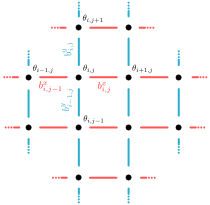
\includegraphics[width=0.7\textwidth]{figures/lattice_implementation.pdf}
\caption{How it is implemented.}
\end{figure}

\underline{Boundary conditions:}\\
\begin{equation}
\intop_{\partial \Omega}b(\bm x)\circ\nabla \theta(\bm x,t)\cdot\bm n\, {\rm d}\bm x  = 0 
\end{equation}
which is trivially true, if
\begin{equation}
n_xb_x\partial_x \theta(\bm x) + n_yb_y\partial_y \theta(\bm x) = 0\,,\; \forall t \text{ and } \bm x \in \partial \Omega \,,
\end{equation}
which leads to
\begin{equation}
\theta_{i,j} = \frac{n_x\big[(n_x+1)b_{i,j-1|i,j}\theta_{i,j-1}+(n_x-1)b_{i,j|i,j+1}\theta_{i,j+1}\big]+
%%
n_y\big[(n_y+1)b_{i-1,j|i,j}\theta_{i-1,j}+(n_y-1)b_{i,j|i+1,j}\theta_{i+1,j}\big]}
%%
{n_x\big[(n_x+1)b_{i,j-1|i,j}+(n_x-1)b_{i,j|i,j+1}\big]+n_y\big[(n_y+1)b_{i-1,j|i,j}+(n_y-1)b_{i,j|i+1,j}\big]}\,,
\end{equation}

\section{Crank-Nicolson}

\begin{equation}
\frac{\Delta t}{2}\,\omega_{ij}(t+\Delta t) + \theta_{ij}(t+\Delta t)=\frac{\Delta t}{2}\,\omega_{ij}(t) + \theta_{ij}(t)
\end{equation}

\begin{equation}
\Big(1+\frac{\gamma_{ij}\Delta t}{2}\Big)\omega_{ij}(t+\Delta t) - \frac{\Delta t}{2}\xi\big(\theta_{ij}(t+\Delta t)\big)
%%
=
%%
\Big(1-\frac{\gamma_{ij}\Delta t}{2}\Big)\omega_{ij}(t)+\frac{\Delta t}{2}\xi\big(\theta_{ij}(t)\big) + (2m_{ij})^{-1}\Big[p_{ij}(t+\Delta t) + p_{ij}(t)\Big]
\end{equation}

\begin{equation}
\left[\begin{array}{cc}
\mathbb{1} & -\frac{\Delta t}{2} \mathbb{1}\\
-\frac{\Delta t}{2}\bm A & \mathbb{1} + \frac{\Delta t}{2}\bm\Gamma
\end{array}\right]\bm x(t+ \Delta t)
%%
=
%%
\left[\begin{array}{cc}
\mathbb{1} & \frac{\Delta t}{2} \mathbb{1}\\
\frac{\Delta t}{2}\bm A & \mathbb{1} - \frac{\Delta t}{2}\bm\Gamma
\end{array}\right]\bm x(t) +
\left[\begin{array}{c}
\mathbb{0}\\
\bm \Pi\end{array}\right]
\end{equation}


\end{document}
